% So we make this "beamer" rather than document!

\documentclass[11pt]{beamer}
% For handout add ,handout after 11pt

\usetheme[sectionpage=none,numbering=none]{metropolis}           % Use metropolis theme
	% To do printouts, add ", handout"  after aspectratio.
\usepackage{booktabs}
\usepackage{graphicx}
\usepackage{color}

\title{Machine Learning Bias}
\author{\small Nick Eubank}
\date{\vspace*{.3in} \date}


% This is the beginning of a real document!
\begin{document}


\begin{frame}
\maketitle
\end{frame}

\begin{frame}[c]{Supervised Machine Learning}
  Conceptual that because Supervised Machine Learning (SML) is built on math, it can't be biased. \\
  SMLs just try to \alert{replicate behavior in training data}. \\
  \pause
  \vspace{0.1cm}
  If training data is biased, algorithm will be too, \emph{even if implemented perfectly!}
\end{frame}

\begin{frame}[c]{Supervised Machine Learning}
  We're building SML model designed to predict performance reviews using resumes.\\
  \pause Train using resumes and performance evaluations of current employees.
  \begin{itemize}
    \pause \item Help decide who to hire.
  \end{itemize}
  \pause
  \vspace{0.1cm}
  If supervisors tend to discriminate against women, then our SML will \alert{look for signals that an applicant is a woman}, since they can use this to give women lower reviews, better matching the training data.
\end{frame}

\begin{frame}[c]{Proxies}
  OK, but what if I don't include data on gender, race, sexuality, etc. in my model? \\
  \vspace{0.1cm}
  \emph{Everything} in society is correlated:
  \begin{itemize}
    \pause \item Going to a women's college (Scripps College, Barnard College)
    \pause \item Going to a Historical Black University (Howard University)
    \pause \item Many activities are gender-correlated (Yoga, Football)
    \pause \item Geography is \emph{extremely} correlated with race and income (Princeton Review)
  \end{itemize}
  \pause In COMPAS, \alert{race wasn't in the model}.
\end{frame}


\begin{frame}[c]{Target an Unbiased Outcome}
\begin{itemize}
  \pause \item In hiring example, variables correlated with gender created bias because the target (performance evaluations) were biased!
\end{itemize}
\pause Less biased targets will reduce the incentive for your algorithm to be biased. \\
\pause Picking unbiased outcomes is not as easy as it seems...
\end{frame}

\begin{frame}[c]{Target an Unbiased Outcome}
  COMPAS: Predicted probability of future arrest. \\
  \pause Arrests are pretty objective, right?
\end{frame}

\begin{frame}[c]{}
  \begin{figure}
    \centering
    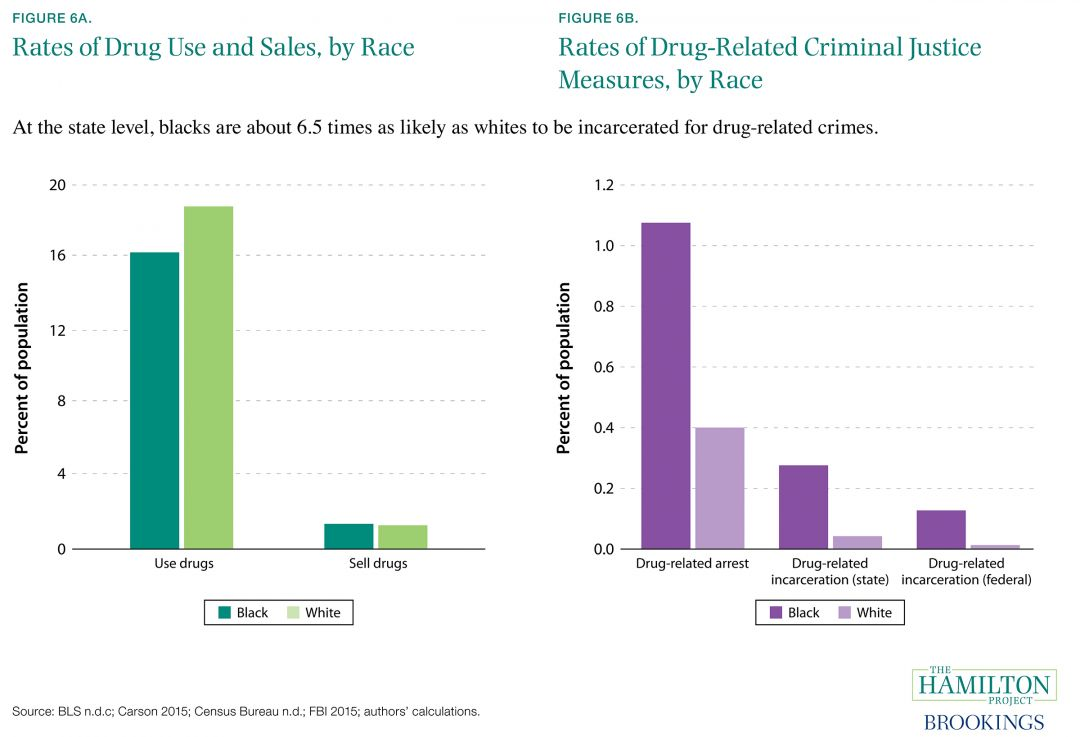
\includegraphics[width=\textwidth]{images/drug_use_versus_arrest.jpg}
  \end{figure}
  Probability of arrest $\neq$ probability of committing a crime
\end{frame}

\begin{frame}[c]{Target an Unbiased Outcome}
    Medical algorithm \alert{thought} future spending on treatments was unbiased \\
    \vspace{0.2cm}
    \pause The relationship between actual ailments and spending varies by race!
\end{frame}

\begin{frame}[c]{Supervised Machine Learning}
  SML models are designed to find any patterns they can to help predict outcomes / classify records. \\
  \vspace{0.2cm}
  \pause Because sexism, racism, xenophobia, homophobia, etc. shape outcomes in the world, \\
  \vspace{0.2cm}
  \pause $\leadsto$ SMLs generally \alert{perform better} when they are sexist/racist/xenophobic/homophobic!
\end{frame}


\begin{frame}[c]{Biased By Design}
  Bias in Machine Learning isn't the result of negligence. \\
  \vspace{0.3cm}
  \pause \alert{So long as society has biases}, Machine Learning has an \alert{affirmative incentive} to be biased too!
\end{frame}

\end{document}
